
\documentclass[10pt,a4paper]{report}
%\usepackage[latin1]{inputenc}
\usepackage[utf8]{inputenc}
\usepackage{amsmath}
\usepackage{amsfonts}
\usepackage{amssymb}
\usepackage{graphicx}
\usepackage{multicol}
\usepackage{tabularx}
\usepackage{mathtools}
\usepackage{tikz}
\usetikzlibrary{arrows,shapes,automata,petri,positioning,calc}
\usepackage{hyperref}
\usepackage{tikz}
\usetikzlibrary{matrix,calc}
\usepackage[margin=0.5in]{geometry}
% ---- power functions -----% 
\newcommand{\myvec}[1]{\ensuremath{\begin{pmatrix}#1\end{pmatrix}}}
\let\vec\mathbf

\providecommand{\norm}[1]{\left\lVert#1\right\rVert}
\providecommand{\abs}[1]{\left\vert#1\right\vert}
\let\vec\mathbf

\newcommand{\mydet}[1]{\ensuremath{\begin{vmatrix}#1\end{vmatrix}}}
\providecommand{\brak}[1]{\ensuremath{\left(#1\right)}}
\providecommand{\lbrak}[1]{\ensuremath{\left(#1\right.}}
\providecommand{\rbrak}[1]{\ensuremath{\left.#1\right)}}
\providecommand{\sbrak}[1]{\ensuremath{{}\left[#1\right]}}
%-------end power functions----%
\newenvironment{Figure}
  {\par\medskip\noindent\minipage{\linewidth}}
  {\endminipage\par\medskip}
\begin{document}
%--------------------logo figure-------------------------%
\begin{figure*}[!tbp]
  \centering
  \begin{minipage}[b]{0.4\textwidth}
%\includegraphics[scale=0.06]{../../../../Downloads/iitlogo.jpg} 
  \end{minipage}
  \hfill
  \vspace{5mm}\begin{minipage}[b]{0.4\textwidth}
%\raggedleft  \includegraphics[scale=0.1]{../../../../Downloads/nrc.jpeg}  

  \end{minipage}\vspace{0.2cm}
\end{figure*}
%--------------------name & rollno-----------------------
\raggedright \textbf{Name}:\hspace{1mm} Ballepu dheeraj kumar\hspace{3cm} \Large \textbf{Assignment-7}\hspace{2.5cm} % 
\normalsize \textbf{Roll No.} :\hspace{1mm} FWC22008\vspace{1cm}
\begin{multicols}{2}

%----------------problem statement--------------%
\raggedright \textbf{Problem Statement:}\vspace{2mm}
\raggedright \\Find the maximum area of a triangle which can be inscribed in a given circle \\
\vspace{5mm}
\section{Solution}
	\begin{flushleft}
Given function is,\\
\end{flushleft} 
    \begin{align}
	\label{eq:vol_varx}
	f(x) = 2x^3r-x^4
	\end{align}
	\textbf{Objective function:}
	\begin{align}
	f(x)=\max_x 2x^3r-x^4
        \end{align}
	\textbf{constraints:}\\
	\begin{align}
		x>0
	\end{align}

	\subsection{Calculation using normal differentiation}
\begin{flushleft}
Differentiating (1) yields,
\end{flushleft}
\begin{align}
\nabla f(x) =6x^2r-4x^3
\end{align}
\begin{flushleft}
\subsection{Calculation of Maxima using gradient ascent algorithm}
\end{flushleft}
\begin{flushleft}
Maxima of the above equation (1), can be calculated from the following expression,\\
\end{flushleft}
%we have to attain the maximum value of area of triangle. This can be seen in Figure.Using gradient ascent method we can find its maxima.
\begin{equation}
        x_{n+1} = x_n + \alpha \nabla f(x_n) 
\end{equation}
\begin{flushleft}
\subsection{Calculation of Maxima using gradient ascent algorithm}
\end{flushleft}
\begin{align}
f(x) = 2x^3r-x^4\\
f'(x) =6x^2r-4x^3
\end{align}
%\begin{equation}
%	x_{n-1} = x_n - \alpha \nabla f(x_n)  
%\end{equation}
\vspace{1mm}
we have to attain the maximum value of area of triangle. This can be seen in Figure.Using gradient ascent method we can find its maxima.
\begin{equation}
\implies x_{n+1}=x_n+\alpha(6x^2r-4x^3)
\end{equation}

Taking $x_0=1,\alpha=0.001$ and precision = 0.00000001, values obtained using python are:
    \begin{align}
        \boxed{\text{Maxima} =0.923176}\\     
        \boxed{\text{Maxima Point} = 1.2900}
    \end{align}
    \section{Theoritical proof}
    \begin{equation}
	    area\hspace{2mm} of\hspace{2mm} the\hspace{2mm} triangle=\frac{1}{2}*b*h
\end{equation}
    where b,base of a triangle is 2*R\\
    h is the height\\
    \begin{equation}
    so \hspace{2mm}area \hspace{2mm}of \hspace{2mm}triangle \hspace{2mm}is \hspace{2mm}R*h
	    \end{equation}
	    \begin{equation}
where R=\sqrt{(r^2-(h-r)^2)}
\end{equation}
r=radius of the circle\\
area being the positive quantity ,A will be maximum if $A^2$ is maximum\\
\begin{equation}
A^2=R^2h^2
\end{equation}
\begin{equation}
Z=R^2h^2
\end{equation}
\begin{equation}
where R^2=2hr-h^2
\end{equation}
%by substituting the above values we get\\
\begin{equation}
Z'=6h^2r-h^4
\end{equation}
for maximum value $Z'=0$\\
by solving the above equation we get\\
    \begin{equation}
	     h=\frac{3}{2}*r
	    %b=$\sqrt{3}$*r\\
    \end{equation}
    $z''$ at h=$\frac{3}{2}$*r is negative\\
    so area is maximum when h=$\frac{3}{2}$*r\\

    by substituting the h value we get\\
    \begin{equation}
	    R=\sqrt{3}*\frac{r}{2}
    \end{equation}
the maximum area of a triangle is obtained at \\
\begin{equation}
	A=\frac{3\sqrt{3}}{4}r^2
\end{equation}


    \section{Conclusion}
\begin{flushleft}
1. At first, the given function has been differentiated and it is solved by setting f'(x) equal to zero. By using x values, f(x) values are calculated.\\
\vspace{0.25cm}
2. Later, the given function f(x) is solved by gradient ascent algorithm to find maxima and the point at which f(x) is maximum.\\
\vspace{0.25cm}
3. Then, the given function f(x) is solved by gradient descent algorithm to find minima and the point at which f(x) is is minimum.\\
\vspace{0.25cm}
\end{flushleft}  
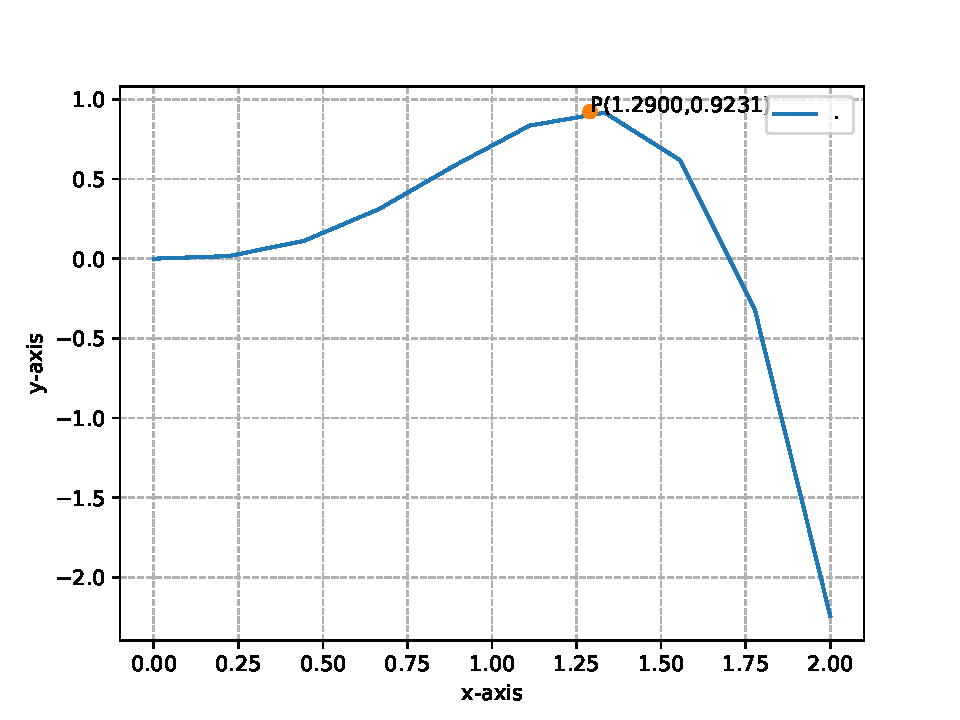
\includegraphics[scale=0.6]{/sdcard/Download/optia/fig/optia.pdf} 
\raggedright  Download the code \\
\url{https://github.com/ballepu1994}
  \end{multicols}
\end{document}
